\documentclass{ximera}

\newcommand{\RR}{\mathbb R}
\renewcommand{\d}{\,d}
\newcommand{\dd}[2][]{\frac{d #1}{d #2}}
\renewcommand{\l}{\ell}
\newcommand{\ddx}{\frac{d}{dx}}
\newcommand{\dfn}{\textbf}
\newcommand{\eval}[1]{\bigg[ #1 \bigg]}


\outcome{Know the graphs and properties of ``famous'' functions.}
\outcome{Understand the properties of trigonometric functions.}
\outcome{Evaluate expressions and solve equations involving
          trigonometric functions and inverse trigonometric functions.}

\title[Dig-In:]{Trigonometric functions}

\begin{document}
\begin{abstract}
  We review trigonometric functions.
\end{abstract}
\maketitle



\section{What are trigonometric functions?}

\begin{definition}
  A \dfn{trigonometric function} is a function that relates a measure
  of an angle of a right triangle to a ratio of the triangle's sides.
\end{definition}


The basic trigonometric functions are cosine and sine. They are called
``trigonometric'' because they relate measures of angles to
measurements of triangles. Given a right triangle
\begin{image}[2in]
  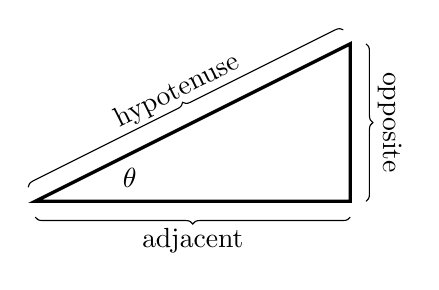
\begin{tikzpicture}
    \coordinate (C) at (0,2);
    \coordinate (D) at (4,2);
    \coordinate (E) at (4,4);
    \tkzMarkRightAngle(C,D,E)
    \tkzMarkAngle(D,C,E)
    \draw[decoration={brace,mirror,raise=.2cm},decorate,thin] (0,2)--(4,2);
    \draw[decoration={brace,mirror,raise=.2cm},decorate,thin] (4,2)--(4,4);
    \draw[decoration={brace,raise=.2cm},decorate,thin] (0,2)--(4,4);
    \draw[very thick] (D)--(E)--(C)--cycle;
    \node at (2,2-.5) {adjacent};
    \node[rotate=-90] at (4+.5,3) {opposite};
    \node[rotate=26.5] at (2-.2,3+.4) {hypotenuse};
    \node at (1.2,2.3) {$\theta$};
  \end{tikzpicture}
\end{image}
we define
\[
\cos(\theta) =
\frac{\text{adjacent}}{\text{hypotenuse}}\qquad\text{and}\qquad\sin(\theta)
= \frac{\text{opposite}}{\text{hypotenuse}}.
\]
Note, the values of sine and cosine do not depend on the scale of the
triangle. Being very explicit, if we scale a triangle by a scale
factor $k$,

\begin{image}[2in]
      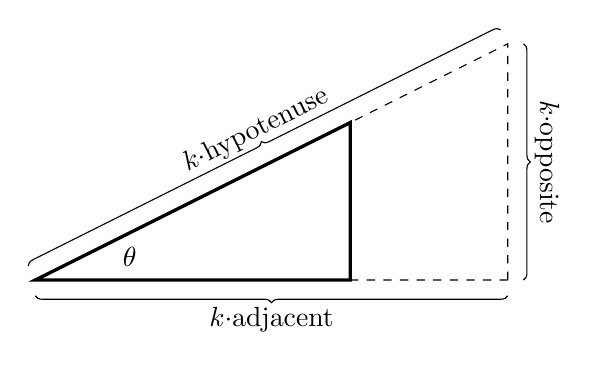
\begin{tikzpicture}
      \coordinate (A) at (6,2);
      \coordinate (B) at (6,5);
      \coordinate (C) at (0,2);
      \coordinate (D) at (4,2);
      \coordinate (E) at (4,4);
      \tkzMarkRightAngle(C,A,B)
      \tkzMarkRightAngle(C,D,E)
      \tkzMarkAngle(D,C,E)
      
      
      \draw[decoration={brace,mirror,raise=.2cm},decorate,thin] (0,2)--(6,2);
      \draw[decoration={brace,mirror,raise=.2cm},decorate,thin] (6,2)--(6,5);
      \draw[decoration={brace,raise=.2cm},decorate,thin] (0,2)--(6,5);
      \draw[dashed] (A)--(B)--(C)--cycle;
      \draw[very thick] (D)--(E)--(C)--cycle;
      \node at (3,2-.5) {\text{$k\cdot$adjacent}};
      \node[rotate=-90] at (6+.5,3.5) {$k\cdot$opposite};
      \node[rotate=26.5] at (3-.2,3.5+.4) {$k\cdot$hypotenuse};
      \node at (1.2,2.3) {$\theta$};
      \end{tikzpicture}
\end{image}
\[
\cos(\theta) = \frac{k\cdot\text{adjacent}}{k\cdot\text{hypotenuse}} =\frac{\text{adjacent}}{\text{hypotenuse}}
\]
and
\[
\sin(\theta) = \frac{k\cdot\text{opposite}}{k\cdot\text{hypotenuse}} = \frac{\text{opposite}}{\text{hypotenuse}}.
\]

At this point we could simply assume that whenever we draw a triangle
for computing sine and cosine, that the hypotenuse will be $1$. We can
do this because we are simply scaling the triangle, and as we see
above, this makes absolutely no difference when computing sine and
cosine. Hence, when the hypotenuse is $1$, we find that a convenient
way to think about sine and cosine is via the unit circle:
\begin{image}
\begin{tikzpicture}
	\begin{axis}[
            xmin=-1.1,xmax=1.1,ymin=-1.1,ymax=1.1,
            axis lines=center,
            width=4in,
            xtick={-1,1},
            ytick={-1,1},
            clip=false,
            unit vector ratio*=1 1 1,
            xlabel=$x$, ylabel=$y$,
            every axis y label/.style={at=(current axis.above origin),anchor=south},
            every axis x label/.style={at=(current axis.right of origin),anchor=west},
          ]        
          \addplot [dashed, smooth, domain=(0:360)] ({cos(x)},{sin(x)}); %% unit circle

          \addplot [textColor] plot coordinates {(0,0) (.766,.643)}; %% 40 degrees

          \addplot [ultra thick,penColor] plot coordinates {(.766,0) (.766,.643)}; %% 40 degrees
          \addplot [ultra thick,penColor2] plot coordinates {(0,0) (.766,0)}; %% 40 degrees
          
          %\addplot [ultra thick,penColor3] plot coordinates {(1,0) (1,.839)}; %% 40 degrees          

          \addplot [textColor,smooth, domain=(0:40)] ({.15*cos(x)},{.15*sin(x)});
          %\addplot [very thick,penColor] plot coordinates {(0,0) (.766,.643)}; %% sector
          %\addplot [very thick,penColor] plot coordinates {(0,0) (1,0)}; %% sector
          %\addplot [very thick, penColor, smooth, domain=(0:40)] ({cos(x)},{sin(x)}); %% sector
          \node at (axis cs:.15,.07) [anchor=west] {$\theta$};
          \node[penColor, rotate=-90] at (axis cs:.84,.322) {$\sin(\theta)$};
          \node[penColor2] at (axis cs:.383,0) [anchor=north] {$\cos(\theta)$};
          %\node[penColor3, rotate=-90] at (axis cs:1.06,.322) {$\tan(\theta)$};
        \end{axis}
\end{tikzpicture}
\end{image}

If we consider all possible combinations of ratios of
\begin{center}
  adjacent, \qquad opposite, \qquad hypotenuse,
\end{center}
(allowing the adjacent and opposite to be negative, as on the unit
circle) we obtain all of the trigonometric functions.

\begin{definition}
  \index{sine}
  \index{cosine}
  \index{tangent}
  \index{secant}
  \index{cosecant}
  \index{cotangent}
  The trigonometric functions\index{trigonometric function} are:
  \[
  \begin{aligned}
  \cos(\theta) &= \frac{\text{adj}}{\text{hyp}}\\
  \sec(\theta) &= \frac{1}{\cos(\theta)}\\
  \tan(\theta) &= \frac{\sin(\theta)}{\cos(\theta)}\qquad
  \end{aligned}
  \qquad
  \begin{aligned}
  \sin(\theta) &= \frac{\text{opp}}{\text{hyp}}\\
  \csc(\theta) &= \frac{1}{\sin(\theta)}\\
  \cot(\theta) &= \frac{\cos(\theta)}{\sin(\theta)}    
  \end{aligned}
  \]
  where the domain of sine and cosine is all real numbers, and the
  other trigonometric functions are defined precisely when their
  denominators are nonzero.
\end{definition}

\begin{question}
  Which of the following expressions are equal to $\sec(\theta)$?
  \begin{selectAll}
    \choice[correct]{$\frac{1}{\cos(\theta)}$}
    \choice{$\frac{1}{\sin(\theta)}$}
    \choice{$\frac{\text{adj}}{\text{hyp}}$}
    \choice[correct]{$\frac{\text{hyp}}{\text{adj}}$}
    \choice[correct]{$\frac{\tan(\theta)}{\sin(\theta)}$}
    \choice[correct]{$\frac{1}{\sin(\theta)\cdot\cot(\theta)}$}
  \end{selectAll}
\end{question}


  
\section{Connections to inverse functions}




Trigonometric functions arise frequently in problems, and often we are
interested in finding specific angle measures.  For instance, you may
want to find some angle $\theta$ such that
\[
\cos(\theta) = .7
\]
Hence we want to be able to ``undo'' trigonometric functions. However, since
trigonometric functions are not one-to-one, meaning there are are
infinitely many angles with $\cos(\theta) = .7$, it is impossible to
find a true inverse function for $\cos(\theta)$. Nevertheless, it is
useful to have something like an inverse to these functions, however
imperfect. The usual approach is to pick out some collection of angles
that produce all possible values exactly once. If we ``discard'' all
other angles, the resulting function has a proper inverse.  In other
words, we are restricting the domain of the trigonometric function in
order to find an inverse.  The function $\cos(\theta)$ takes on all
values between $-1$ and $1$ exactly once on the interval $[0,\pi]$.

\begin{image}
\begin{tikzpicture}
	\begin{axis}[
            xmin=-6.75,xmax=6.75,ymin=-1.5,ymax=1.5,
            axis lines=center,
            xtick={-6.28, -4.71, -3.14, -1.57, 0, 1.57, 3.142, 4.71, 6.28},
            xticklabels={$-2\pi$,$-3\pi/2$,$-\pi$, $-\pi/2$, $0$, $\pi/2$, $\pi$, $3\pi/2$, $2\pi$},
            ytick={-1,1},
            %ticks=none,
            width=6in,
            height=3in,
            unit vector ratio*=1 1 1,
            xlabel=$\theta$, ylabel=$x$,
            every axis y label/.style={at=(current axis.above origin),anchor=south},
            every axis x label/.style={at=(current axis.right of origin),anchor=west},
          ]        
          \addplot [very thick, penColor2!20!background, samples=100,smooth, domain=(-6.75:0)] {cos(deg(x))};
          \addplot [very thick, penColor2!20!background, samples=100,smooth, domain=(3.14:6.75)] {cos(deg(x))};
          \addplot [very thick, penColor2, samples=100,smooth, domain=(0:3.14)] {cos(deg(x))};
          
          \addplot[color=penColor2,fill=penColor2,only marks,mark=*] coordinates{(0,1)};  %% closed hole          
          \addplot[color=penColor2,fill=penColor2,only marks,mark=*] coordinates{(pi,-1)};  %% closed hole          
          \node at (axis cs:-1.57,.75) [penColor2] {$\cos(\theta)$};
        \end{axis}
\end{tikzpicture}
%% \caption{The function $\cos(\theta)$ takes on all values between $-1$
%%   and $1$ exactly once on the interval $[0,\pi]$. If we restrict
%%   $\cos(\theta)$ to this interval, then this restricted function has
%%   an inverse.}
%% \label{figure:cos-restricted}
%% \end{figure*}
\end{image}
If we restrict the domain of $\cos(\theta)$ to this interval, then this
restricted function is one-to-one and hence has an inverse.

\begin{question}
  What arc on the unit circle corresponds to the restricted domain
  described above of $\cos(\theta)$?
  \begin{multipleChoice}
    \choice{\begin{tikzpicture}[framed,scale=.2,baseline=4ex]
	\begin{axis}[
            xmin=-1.1,xmax=1.1,ymin=-1.1,ymax=1.1,
            axis lines=center,
            width=4in,
            ticks=none,
            clip=false,
            unit vector ratio*=1 1 1,
            %xlabel=$x$, ylabel=$y$,
            every axis y label/.style={at=(current axis.above origin),anchor=south},
            every axis x label/.style={at=(current axis.right of origin),anchor=west},
          ]        
          \addplot [dashed, smooth, domain=(0:360)] ({cos(x)},{sin(x)}); %% unit circle

          \addplot [line width=2mm,penColor2, domain=(-90:90)] ({cos(x)},{sin(x)}); %% unit circle
        \end{axis}
    \end{tikzpicture}}
    \choice[correct]{\begin{tikzpicture}[framed,scale=.2,baseline=4ex]
	\begin{axis}[
            xmin=-1.1,xmax=1.1,ymin=-1.1,ymax=1.1,
            axis lines=center,
            width=4in,
            ticks=none,
            clip=false,
            unit vector ratio*=1 1 1,
            %xlabel=$x$, ylabel=$y$,
            every axis y label/.style={at=(current axis.above origin),anchor=south},
            every axis x label/.style={at=(current axis.right of origin),anchor=west},
          ]        
          \addplot [dashed, smooth, domain=(0:360)] ({cos(x)},{sin(x)}); %% unit circle

          \addplot [line width=2mm,penColor2, domain=(0:180)] ({cos(x)},{sin(x)}); %% unit circle
        \end{axis}
    \end{tikzpicture}}
    \choice{\begin{tikzpicture}[framed,scale=.2,baseline=4ex]
	\begin{axis}[
            xmin=-1.1,xmax=1.1,ymin=-1.1,ymax=1.1,
            axis lines=center,
            width=4in,
            ticks=none,
            clip=false,
            unit vector ratio*=1 1 1,
            %xlabel=$x$, ylabel=$y$,
            every axis y label/.style={at=(current axis.above origin),anchor=south},
            every axis x label/.style={at=(current axis.right of origin),anchor=west},
          ]        
          \addplot [dashed, smooth, domain=(0:360)] ({cos(x)},{sin(x)}); %% unit circle

          \addplot [line width=2mm,penColor2, domain=(90:270)] ({cos(x)},{sin(x)}); %% unit circle
        \end{axis}
    \end{tikzpicture}}
    \choice{\begin{tikzpicture}[framed,scale=.2,baseline=4ex]
	\begin{axis}[
            xmin=-1.1,xmax=1.1,ymin=-1.1,ymax=1.1,
            axis lines=center,
            width=4in,
            ticks=none,
            clip=false,
            unit vector ratio*=1 1 1,
            %xlabel=$x$, ylabel=$y$,
            every axis y label/.style={at=(current axis.above origin),anchor=south},
            every axis x label/.style={at=(current axis.right of origin),anchor=west},
          ]        
          \addplot [dashed, smooth, domain=(0:360)] ({cos(x)},{sin(x)}); %% unit circle

          \addplot [line width=2mm,penColor2, domain=(180:360)] ({cos(x)},{sin(x)}); %% unit circle
        \end{axis}
\end{tikzpicture}}
  \end{multipleChoice}
\end{question}



In a similar fashion, we need to restrict the domain of sine to be able
to take an inverse. The function $\sin(\theta)$ takes on all values
between $-1$ and $1$ exactly once on the interval $[-\pi/2,\pi/2]$.

\begin{image}
\begin{tikzpicture}
	\begin{axis}[
            xmin=-6.75,xmax=6.75,ymin=-1.5,ymax=1.5,
            axis lines=center,
            xtick={-6.28, -4.71, -3.14, -1.57, 0, 1.57, 3.142, 4.71, 6.28},
            xticklabels={$-2\pi$,$-3\pi/2$,$-\pi$, $-\pi/2$, $0$, $\pi/2$, $\pi$, $3\pi/2$, $2\pi$},
            ytick={-1,1},
            %ticks=none,
            width=6in,
            height=3in,
            unit vector ratio*=1 1 1,
            xlabel=$\theta$, ylabel=$x$,
            every axis y label/.style={at=(current axis.above origin),anchor=south},
            every axis x label/.style={at=(current axis.right of origin),anchor=west},
          ]        
          \addplot [very thick, penColor!20!background, samples=100,smooth, domain=(-6.75:-1.57)] {sin(deg(x))};
          \addplot [very thick, penColor!20!background, samples=100,smooth, domain=(1.57:6.75)] {sin(deg(x))};
          \addplot [very thick, penColor, samples=100,smooth, domain=(-1.57:1.57)] {sin(deg(x))};
          
          \addplot[color=penColor,fill=penColor,only marks,mark=*] coordinates{(-1.57,-1)};  %% closed hole          
          \addplot[color=penColor,fill=penColor,only marks,mark=*] coordinates{(1.57,1)};  %% closed hole          
          \node at (axis cs:3.14,.75) [penColor] {$\sin(\theta)$};
        \end{axis}
\end{tikzpicture}
%% \caption{The function $\sin(\theta)$ takes on all values between $-1$
%%   and $1$ exactly once on the interval $[-\pi/2,\pi/2]$. If we
%%   restrict $\sin(\theta)$ to this interval, then this restricted
%%   function has an inverse.}
%% \label{figure:sin-restricted}
%% \end{figure*}
\end{image}



If we restrict the domain of $\sin(\theta)$ to this interval, then this restricted
function is one-to-one and thus has an inverse.

\begin{question}
  What arc on the unit circle corresponds to the restricted domain described above of
  $\sin(\theta)$?
  \begin{multipleChoice}
    \choice[correct]{\begin{tikzpicture}[framed,scale=.2,baseline=4ex]
	\begin{axis}[
            xmin=-1.1,xmax=1.1,ymin=-1.1,ymax=1.1,
            axis lines=center,
            width=4in,
            ticks=none,
            clip=false,
            unit vector ratio*=1 1 1,
            %xlabel=$x$, ylabel=$y$,
            every axis y label/.style={at=(current axis.above origin),anchor=south},
            every axis x label/.style={at=(current axis.right of origin),anchor=west},
          ]        
          \addplot [dashed, smooth, domain=(0:360)] ({cos(x)},{sin(x)}); %% unit circle

          \addplot [line width=2mm,penColor, domain=(-90:90)] ({cos(x)},{sin(x)}); %% unit circle
        \end{axis}
    \end{tikzpicture}}
    \choice{\begin{tikzpicture}[framed,scale=.2,baseline=4ex]
	\begin{axis}[
            xmin=-1.1,xmax=1.1,ymin=-1.1,ymax=1.1,
            axis lines=center,
            width=4in,
            ticks=none,
            clip=false,
            unit vector ratio*=1 1 1,
            %xlabel=$x$, ylabel=$y$,
            every axis y label/.style={at=(current axis.above origin),anchor=south},
            every axis x label/.style={at=(current axis.right of origin),anchor=west},
          ]        
          \addplot [dashed, smooth, domain=(0:360)] ({cos(x)},{sin(x)}); %% unit circle

          \addplot [line width=2mm,penColor, domain=(0:180)] ({cos(x)},{sin(x)}); %% unit circle
        \end{axis}
    \end{tikzpicture}}
    \choice{\begin{tikzpicture}[framed,scale=.2,baseline=4ex]
	\begin{axis}[
            xmin=-1.1,xmax=1.1,ymin=-1.1,ymax=1.1,
            axis lines=center,
            width=4in,
            ticks=none,
            clip=false,
            unit vector ratio*=1 1 1,
            %xlabel=$x$, ylabel=$y$,
            every axis y label/.style={at=(current axis.above origin),anchor=south},
            every axis x label/.style={at=(current axis.right of origin),anchor=west},
          ]        
          \addplot [dashed, smooth, domain=(0:360)] ({cos(x)},{sin(x)}); %% unit circle

          \addplot [line width=2mm,penColor, domain=(90:270)] ({cos(x)},{sin(x)}); %% unit circle
        \end{axis}
    \end{tikzpicture}}
    \choice{\begin{tikzpicture}[framed,scale=.2,baseline=4ex]
	\begin{axis}[
            xmin=-1.1,xmax=1.1,ymin=-1.1,ymax=1.1,
            axis lines=center,
            width=4in,
            ticks=none,
            clip=false,
            unit vector ratio*=1 1 1,
            %xlabel=$x$, ylabel=$y$,
            every axis y label/.style={at=(current axis.above origin),anchor=south},
            every axis x label/.style={at=(current axis.right of origin),anchor=west},
          ]        
          \addplot [dashed, smooth, domain=(0:360)] ({cos(x)},{sin(x)}); %% unit circle

          \addplot [line width=2mm,penColor, domain=(180:360)] ({cos(x)},{sin(x)}); %% unit circle
        \end{axis}
\end{tikzpicture}}
  \end{multipleChoice}
\end{question}



By examining both sine and cosine on restricted domains, we can now produce functions arcsine and arccosine:

\begin{image}[2in]\index{arccosine}
\begin{tikzpicture}
	\begin{axis}[
            xmin=-1.5,xmax=1.5,ymin=-.25,ymax=3.25,
            axis lines=center,
            ytick={0, 1.57,3.14},
            yticklabels={$0$, $\pi/2$,$\pi$},
            xtick={-1,1},
            unit vector ratio*=1 1 1,
            xlabel=$x$, ylabel=$\theta$,
            every axis y label/.style={at=(current axis.above origin),anchor=south},
            every axis x label/.style={at=(current axis.right of origin),anchor=west},
          ]        
          \addplot [very thick, penColor5, samples=100,smooth, domain=(-1:1)] {acos(x)*pi/180};
          \addplot[color=penColor5,fill=penColor5,only marks,mark=*] coordinates{(1,0)};  %% closed hole          
          \addplot[color=penColor5,fill=penColor5,only marks,mark=*] coordinates{(-1,pi)};  %% closed hole
        \end{axis}
        \node at (3,-1) [text width=2.75in] {Here we see a plot of $\arccos(x)$, the inverse function of
          $\cos(\theta)$ when the domain is restricted to the interval $[0,\pi]$.};
\end{tikzpicture} 
\end{image}
\begin{image}[2in]\index{arcsine}
\begin{tikzpicture}
	\begin{axis}[
            xmin=-1.5,xmax=1.5,ymin=-1.75,ymax=1.75,
            axis lines=center,
            ytick={-1.57, 0, 1.57},
            yticklabels={$-\pi/2$, $0$, $\pi/2$},
            xtick={-1,1},
            unit vector ratio*=1 1 1,
            xlabel=$x$, ylabel=$\theta$,
            every axis y label/.style={at=(current axis.above origin),anchor=south},
            every axis x label/.style={at=(current axis.right of origin),anchor=west},
          ]        
          \addplot [very thick, penColor4, samples=100,smooth, domain=(-1:1)] {asin(x)*pi/180};
                    
          \addplot[color=penColor4,fill=penColor4,only marks,mark=*] coordinates{(-1,-pi/2)};  %% closed hole          
          \addplot[color=penColor4,fill=penColor4,only marks,mark=*] coordinates{(1,pi/2)};  %% closed hole
        \end{axis}
        \node at (3,-1) [text width=2.75in] {Here we see a plot of $\arcsin(x)$, the inverse function of
$\sin(\theta)$ when the domain is restricted to the interval $[-\pi/2,\pi/2]$.};
\end{tikzpicture} 
\end{image}

The functions
\[
\arccos(x)\qquad\text{and}\qquad\arcsin(x)
\]
are called ``arc'' because they give the angle that cosine or sine
used to produce their value.  It is quite common to write
\[
\arccos(x) = \cos^{-1}(x)\qquad\text{and}\qquad\arcsin(x) = \sin^{-1}(x).
\]
However, this notation is misleading as $\cos^{-1}(x)$ and
$\sin^{-1}(x)$ are not true inverse functions of cosine and sine.
Recall that a function and its inverse undo each other in either
order, for example,
\[
\sqrt[3]{x^3}=x\qquad \text{and}\qquad \left(\sqrt[3]{x}\right)^3=x. 
\]
Since arcsine is the inverse of sine restricted to the interval
$[-\pi/2,\pi/2]$, this does not work with sine and arcsine, for
example
\[
\arcsin(\sin(\pi))=0.
\]
though it is true that
\[
\sin(\arcsin(x)) = x\qquad\text{and}\qquad\cos(\arccos(x)) = x.
\]
\begin{question}
   Which of the following statements is true?
   \begin{multipleChoice}
     \choice{$\sin^{-1}(x)$ is the inverse function of $\sin(x)$} %this is perhaps a bit too subtle?
     \choice[correct]{$\sin\left(\sin^{-1}\left(\frac{1}{2}\right)\right) = \frac{1}{2}$} 
     \choice{$\sin^{-1}\left(\sin\left(\frac{5\pi}{2}\right)\right) = \frac{5\pi}{2}$}
     \choice{$\sin^{-1}(x) = \frac{1}{\sin(x)}$}
   \end{multipleChoice}  
\end{question}



\begin{example}
  Compute:
  \[
  \arccos(\cos(5\pi/3))
  \]
  \begin{explanation}
    The issue here is that $5\pi/3$ might not be in the range of
    arccosine. To find our missing number, we'll check with a unit
    circle that we've decorated with the domain of arccosine:
\begin{image}
\begin{tikzpicture}
	\begin{axis}[
            xmin=-1.1,xmax=1.1,ymin=-1.1,ymax=1.1,
            axis lines=center,
            width=4in,
            ticks=none,
            clip=false,
            unit vector ratio*=1 1 1,
            xlabel=$x$, ylabel=$y$,
            every axis y label/.style={at=(current axis.above origin),anchor=south},
            every axis x label/.style={at=(current axis.right of origin),anchor=west},
          ]        
          \addplot [dashed, smooth, domain=(0:360)] ({cos(x)},{sin(x)}); %% unit circle
          \addplot [very thick, color=penColor2, smooth, domain=(0:180)] ({cos(x)},{sin(x)}); %% domain
          \addplot[color=penColor2,fill=penColor2,only marks,mark=*] coordinates{({cos(60)},{sin(60)})};  %% closed hole
          \addplot[color=penColor2,fill=penColor2,only marks,mark=*] coordinates{({cos(120)},{sin(120)})};  %% closed hole
          \addplot[color=penColor2,fill=penColor2,only marks,mark=*] coordinates{({cos(180)},{sin(180)})};  %% closed hole
          \addplot[only marks,mark=*] coordinates{({cos(240)},{sin(240)})};  %% closed hole
          \addplot[only marks,mark=*] coordinates{({cos(300)},{sin(300)})};  %% closed hole
          \addplot[color=penColor2,fill=penColor2,only marks,mark=*] coordinates{({cos(360)},{sin(360)})};  %% closed hole

          \node at (axis cs:{(1,0)}) [anchor=south west,penColor2] {$0$};
          \node at (axis cs:{cos(60)},{sin(60)}) [anchor=south west,penColor2] {$\pi/3$};
          \node at (axis cs:{cos(120)},{sin(120)}) [anchor=south east,penColor2] {$2\pi/3$};
          \node at (axis cs:{cos(180)},{sin(180)}) [anchor=south east,penColor2] {$\pi$};
          
          \node at (axis cs:{cos(60)},{sin(60)}) [anchor=north east] {$\pi/3$};
          \node at (axis cs:{cos(120)},{sin(120)}) [anchor=north west] {$2\pi/3$};
          \node at (axis cs:{cos(180)},{sin(180)}) [anchor=north west] {$\pi$};
          \node at (axis cs:{cos(240)},{sin(240)}) [anchor=south west] {$4\pi/3$};
          \node at (axis cs:{cos(300)},{sin(300)}) [anchor=south east] {$5\pi/3$};
          %\node at (axis cs:{cos(360)},{sin(360)}) [anchor=north east] {$2\pi$};
        \end{axis}          
\end{tikzpicture}
\end{image}
Since the points $5\pi/3$ and $\pi/3$ have the same $x$-coordinate,
$\cos(5\pi/3) = \cos(\pi/3)$. Hence
\[
\arccos(\cos(5\pi/3)) = \pi/3.
\]
  \end{explanation}
\end{example}


Now that you have a feel for how $\arcsin(x)$ and $\arccos(x)$ behave, let's examine tangent.

\begin{image}
\begin{tikzpicture}
	\begin{axis}[
            xmin=-6.75,xmax=6.75,ymin=-3,ymax=3,
            axis lines=center,
            width=6in,
            height=3in,
            xtick={-6.28, -4.71, -3.14, -1.57, 0, 1.57, 3.142, 4.71, 6.28},
            xticklabels={$-2\pi$,$-3\pi/2$,$-\pi$, $-\pi/2$, $0$, $\pi/2$, $\pi$, $3\pi/2$, $2\pi$},       
            unit vector ratio*=1 1 1,
            xlabel=$\theta$, ylabel=$x$,
            every axis y label/.style={at=(current axis.above origin),anchor=south},
            every axis x label/.style={at=(current axis.right of origin),anchor=west},
          ]        
          \addplot [very thick, penColor3, samples=100,smooth, domain=(-1.55:1.55)] {tan(deg(x))};
          \addplot [very thick, penColor3!30!background, samples=100,smooth, domain=(-4.69:-1.59)] {tan(deg(x))};
          \addplot [very thick, penColor3!30!background, samples=100,smooth, domain=(-6.75:-4.73)] {tan(deg(x))};
          \addplot [very thick, penColor3!30!background, samples=100,smooth, domain=(1.59:4.69)] {tan(deg(x))};
          \addplot [very thick, penColor3!30!background, samples=100,smooth, domain=(4.73:6.75)] {tan(deg(x))};
          
          \addplot [textColor,dashed] plot coordinates {(-4.71,-3) (-4.71,3)};
          \addplot [textColor,dashed] plot coordinates {(-1.57,-3) (-1.57,3)};
          \addplot [textColor,dashed] plot coordinates {(1.57,-3) (1.57,3)};
          \addplot [textColor,dashed] plot coordinates {(4.71,-3) (4.71,3)};
          
          \node at (axis cs:.4,1.25) [penColor3] {$\tan(\theta)$};    
        \end{axis}
\end{tikzpicture}
%% \caption{The function $\tan(\theta)$ takes on all values in $\R$
%%   exactly once on the open interval $(-\pi/2,\pi/2)$. If we restrict
%%   $\tan(\theta)$ to this interval, then this restricted function has
%%   an inverse.}
%% \end{figure*}
%% \end{fullwidth}
\end{image}
  \begin{question}
  What arc on the unit circle corresponds to the restricted domain described above of
  $\tan(\theta)$?
  \begin{multipleChoice}
    \choice[correct]{\begin{tikzpicture}[framed,scale=.2,baseline=4ex]
	\begin{axis}[
            xmin=-1.1,xmax=1.1,ymin=-1.1,ymax=1.1,
            axis lines=center,
            width=4in,
            ticks=none,
            clip=false,
            unit vector ratio*=1 1 1,
            %xlabel=$x$, ylabel=$y$,
            every axis y label/.style={at=(current axis.above origin),anchor=south},
            every axis x label/.style={at=(current axis.right of origin),anchor=west},
          ]        
          \addplot [dashed, smooth, domain=(0:360)] ({cos(x)},{sin(x)}); %% unit circle

          \addplot [line width=2mm,penColor3, domain=(-90:90)] ({cos(x)},{sin(x)}); %% unit circle
        \end{axis}
    \end{tikzpicture}}
    \choice{\begin{tikzpicture}[framed,scale=.2,baseline=4ex]
	\begin{axis}[
            xmin=-1.1,xmax=1.1,ymin=-1.1,ymax=1.1,
            axis lines=center,
            width=4in,
            ticks=none,
            clip=false,
            unit vector ratio*=1 1 1,
            %xlabel=$x$, ylabel=$y$,
            every axis y label/.style={at=(current axis.above origin),anchor=south},
            every axis x label/.style={at=(current axis.right of origin),anchor=west},
          ]        
          \addplot [dashed, smooth, domain=(0:360)] ({cos(x)},{sin(x)}); %% unit circle

          \addplot [line width=2mm,penColor3, domain=(0:180)] ({cos(x)},{sin(x)}); %% unit circle
        \end{axis}
    \end{tikzpicture}}
    \choice{\begin{tikzpicture}[framed,scale=.2,baseline=4ex]
	\begin{axis}[
            xmin=-1.1,xmax=1.1,ymin=-1.1,ymax=1.1,
            axis lines=center,
            width=4in,
            ticks=none,
            clip=false,
            unit vector ratio*=1 1 1,
            %xlabel=$x$, ylabel=$y$,
            every axis y label/.style={at=(current axis.above origin),anchor=south},
            every axis x label/.style={at=(current axis.right of origin),anchor=west},
          ]        
          \addplot [dashed, smooth, domain=(0:360)] ({cos(x)},{sin(x)}); %% unit circle

          \addplot [line width=2mm,penColor3, domain=(90:270)] ({cos(x)},{sin(x)}); %% unit circle
        \end{axis}
    \end{tikzpicture}}
    \choice{\begin{tikzpicture}[framed,scale=.2,baseline=4ex]
	\begin{axis}[
            xmin=-1.1,xmax=1.1,ymin=-1.1,ymax=1.1,
            axis lines=center,
            width=4in,
            ticks=none,
            clip=false,
            unit vector ratio*=1 1 1,
            %xlabel=$x$, ylabel=$y$,
            every axis y label/.style={at=(current axis.above origin),anchor=south},
            every axis x label/.style={at=(current axis.right of origin),anchor=west},
          ]        
          \addplot [dashed, smooth, domain=(0:360)] ({cos(x)},{sin(x)}); %% unit circle

          \addplot [line width=2mm,penColor3, domain=(180:360)] ({cos(x)},{sin(x)}); %% unit circle
        \end{axis}
\end{tikzpicture}}
  \end{multipleChoice}
\end{question}
Again, only working on a restricted domain of tangent, we can produce
an inverse function, arctangent. Here we see a plot of $\arctan(x)$,
the inverse function of $\tan(\theta)$ when its domain is restricted to the
interval $(-\pi/2,\pi/2)$.

\begin{image}
\begin{tikzpicture}
	\begin{axis}[
            xmin=-6,xmax=6,ymin=-2,ymax=2,
            axis lines=center,
            ytick={0, -1.57,1.57},
            width=6in,
            height=3in,
            yticklabels={$0$, $-\pi/2$,$\pi/2$},
            xtick={0},
            unit vector ratio*=1 1 1,
            xlabel=$x$, ylabel=$\theta$,
            every axis y label/.style={at=(current axis.above origin),anchor=south},
            every axis x label/.style={at=(current axis.right of origin),anchor=west},
          ]        
          \addplot [very thick, penColor3!20!penColor2, samples=100,smooth, domain=(-6:6)] {atan(x)*pi/180};
          \addplot [textColor,dashed] plot coordinates {(-6,-1.57) (6,-1.57)};
          \addplot [textColor,dashed] plot coordinates {(-6,1.57) (6,1.57)};
        \end{axis}
\end{tikzpicture}
%% \caption{Here we see a plot of $\arctan(y)$, the inverse function of
%% $\tan(\theta)$ when it is restricted to the interval $(-\pi/2,\pi/2)$.}
%% \end{figure*}
%% \index{arctangent}
%% \end{fullwidth}
\end{image}





\begin{example}
  Compute:
  \[
  \arctan(\tan(5\pi/3))
  \]
  \begin{explanation}
    The issue here is that $5\pi/3$ might not be in the range of
    arctangent. To find our missing number, we'll check with a unit
    circle that we've decorated with the domain of arctangent:
\begin{image}
\begin{tikzpicture}
	\begin{axis}[
            xmin=-1.1,xmax=1.1,ymin=-1.1,ymax=1.1,
            axis lines=center,
            width=4in,
            ticks=none,
            clip=false,
            unit vector ratio*=1 1 1,
            xlabel=$x$, ylabel=$y$,
            every axis y label/.style={at=(current axis.above origin),anchor=south},
            every axis x label/.style={at=(current axis.right of origin),anchor=west},
          ]        
          \addplot [dashed, smooth, domain=(0:360)] ({cos(x)},{sin(x)}); %% unit circle
          \addplot [very thick, color=penColor3, smooth, domain=(-90:90)] ({cos(x)},{sin(x)}); %% domain
          \addplot[color=penColor3,fill=penColor3,only marks,mark=*] coordinates{({cos(60)},{sin(60)})};  %% closed hole
          \addplot[only marks,mark=*] coordinates{({cos(120)},{sin(120)})};  %% closed hole
          \addplot[only marks,mark=*] coordinates{({cos(180)},{sin(180)})};  %% closed hole
          \addplot[only marks,mark=*] coordinates{({cos(240)},{sin(240)})};  %% closed hole
          \addplot[color=penColor3, fill=penColor3,only marks,mark=*] coordinates{({cos(300)},{sin(300)})};  %% closed hole
          \addplot[color=penColor3,fill=penColor3,only marks,mark=*] coordinates{({cos(360)},{sin(360)})};  %% closed hole

          \addplot[color=penColor3,fill=white,only marks,mark=*] coordinates{({cos(90)},{sin(90)})};  %% open hole
          \addplot[color=penColor3,fill=white,only marks,mark=*] coordinates{({cos(-90)},{sin(-90)})};  %% open hole

          
          \node at (axis cs:{(1,0)}) [anchor=south west,penColor3] {$0$};
          \node at (axis cs:{cos(60)},{sin(60)}) [anchor=south west,penColor3] {$\pi/3$};
          \node at (axis cs:{cos(300)},{sin(300)}) [anchor=north west,penColor3] {$-\pi/3$};
                    
          \node at (axis cs:{cos(60)},{sin(60)}) [anchor=north east] {$\pi/3$};
          \node at (axis cs:{cos(120)},{sin(120)}) [anchor=north west] {$2\pi/3$};
          \node at (axis cs:{cos(180)},{sin(180)}) [anchor=north west] {$\pi$};
          \node at (axis cs:{cos(240)},{sin(240)}) [anchor=south west] {$4\pi/3$};
          \node at (axis cs:{cos(300)},{sin(300)}) [anchor=south east] {$5\pi/3$};
          %\node at (axis cs:{cos(360)},{sin(360)}) [anchor=north east] {$2\pi$};
        \end{axis}          
\end{tikzpicture}
\end{image}
Since the points $5\pi/3$ and $-\pi/3$ have the same $x$ and $y$-coordinates,
\[
\arctan(\tan(5\pi/3)) = -\pi/3.
\]
  \end{explanation}
\end{example}



Now we give some facts of other trigonometric and ``inverse''
trigonometric functions.

\begin{definition}\hfil
  \index{arccosine}
  \index{arcsine}
  \index{arctangent}
  \index{arcsecant}
  \index{arccosecant}
  \index{arccotangent}
  \index{inverse!trigonometric functions}
  \begin{itemize}
    \item $\arccos(x) = \theta$ means that $\cos(\theta) = x$ and
      $0\le \theta\le \pi$. The domain of $\arccos(x)$ is $-1\le x\le
      1$.
    \item $\arcsin(x) = \theta$ means that $\sin(\theta) = x$ and
      $-\frac{\pi}{2}\le \theta\le \frac{\pi}{2}$. The domain of
      $\arcsin(x)$ is $-1\le x\le 1$.
    \item $\arctan(x) = \theta$ means that $\tan(\theta) = x$ and
      $-\frac{\pi}{2}< \theta< \frac{\pi}{2}$. The domain of
      $\arctan(x)$ is $-\infty<x<\infty$.
    \item $\arccot(x) = \theta$ means that $\cot(\theta) = x$ and
      $0< \theta< \pi$. The domain of $\arccot(x)$ is
      $-\infty<x<\infty$.
    \item $\arcsec(x) = \theta$ means that $\sec(\theta) = x$ and
      $0\le \theta\le \pi$ with $\theta\ne \pi/2$. The domain of
      $\arcsec(x)$ is all $x$ with absolute value greater than $1$.
    \item $\arccsc(x) = \theta$ means that $\csc(\theta) = x$ and
      $-\frac{\pi}{2}\le \theta\le \frac{\pi}{2}$ with $\theta \ne 0$. The
      domain of $\arccsc(x)$ is all $x$ with absolute value greater
      than $1$.
  \end{itemize}
\end{definition}


\section{The power of the Pythagorean Theorem}

The Pythagorean Theorem is probably the most famous theorem in all of
mathematics.


\begin{theorem}[Pythagorean Theorem]\index{Pythagorean Theorem}
Given a right triangle:
\begin{image}[2in]
  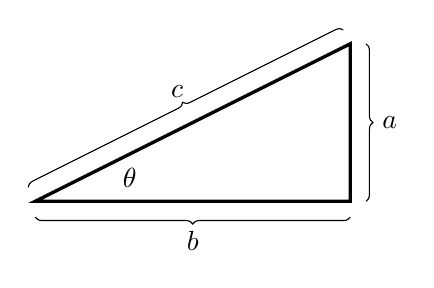
\begin{tikzpicture}
    \coordinate (C) at (0,2);
    \coordinate (D) at (4,2);
    \coordinate (E) at (4,4);
    \tkzMarkRightAngle(C,D,E)
    \tkzMarkAngle(D,C,E)
    \draw[decoration={brace,mirror,raise=.2cm},decorate,thin] (0,2)--(4,2);
    \draw[decoration={brace,mirror,raise=.2cm},decorate,thin] (4,2)--(4,4);
    \draw[decoration={brace,raise=.2cm},decorate,thin] (0,2)--(4,4);
    \draw[very thick] (D)--(E)--(C)--cycle;
    \node at (2,2-.5) {$b$};
    \node[] at (4+.5,3) {$a$};
    \node at (2-.2,3+.4) {$c$};
    \node at (1.2,2.3) {$\theta$};
  \end{tikzpicture}
\end{image}
We have that:
\[
a^2 + b^2 = c^2
\]
\end{theorem}


The Pythagorean Theorem gives several key trigonometric identities.

\begin{theorem}[Pythagorean Identities]\index{Pythagorean identities}
  The following hold:
  \[
  \cos^2\theta+\sin^2\theta = 1 \qquad 1 + \tan^2\theta = \sec^2\theta \qquad \cot^2\theta + 1 = \csc^2\theta
  \]
  \begin{explanation}
    From the unit circle we can see
    \begin{image}
\begin{tikzpicture}
	\begin{axis}[
            xmin=-1.1,xmax=1.1,ymin=-1.1,ymax=1.1,
            axis lines=center,
            width=4in,
            ticks=none,
            clip=false,
            unit vector ratio*=1 1 1,
            %xlabel=$x$, ylabel=$y$,
            every axis y label/.style={at=(current axis.above origin),anchor=south},
            every axis x label/.style={at=(current axis.right of origin),anchor=west},
          ]        
          \addplot [dashed, smooth, domain=(0:360)] ({cos(x)},{sin(x)}); %% unit circle

          \addplot [textColor] plot coordinates {(0,0) (.766,.643)}; %% 40 degrees

          \addplot [ultra thick,penColor] plot coordinates {(.766,0) (.766,.643)}; %% 40 degrees
          \addplot [ultra thick,penColor2] plot coordinates {(0,0) (.766,0)}; %% 40 degrees
          
          %\addplot [ultra thick,penColor3] plot coordinates {(1,0) (1,.839)}; %% 40 degrees          

          \addplot [textColor,smooth, domain=(0:40)] ({.15*cos(x)},{.15*sin(x)});
          %\addplot [very thick,penColor] plot coordinates {(0,0) (.766,.643)}; %% sector
          %\addplot [very thick,penColor] plot coordinates {(0,0) (1,0)}; %% sector
          %\addplot [very thick, penColor, smooth, domain=(0:40)] ({cos(x)},{sin(x)}); %% sector
          \node at (axis cs:.15,.07) [anchor=west] {$t$};
          \node[penColor, rotate=-90] at (axis cs:.84,.322) {$\sin(t)$};
          \node[penColor2] at (axis cs:.383,0) [anchor=north] {$\cos(t)$};
          %\node[penColor3, rotate=-90] at (axis cs:1.06,.322) {$\tan(\theta)$};
        \end{axis}
\end{tikzpicture}
    \end{image}
    via the Pythagorean Theorem that
    \[
    \cos^2(t) + \sin^2(t) = 1.
    \]
    If we divide this expression by $\answer[given]{\cos^2(t)}$ we obtain
    \[
    1 + \tan^2(t) = \sec^2(t)
    \]
    and if we divide $\cos^2(t) + \sin^2(t) = 1$ by $\answer[given]{\sin^2(t)}$ we obtain
    \[
    \cot^2(t) + 1 = \csc^2(t).
    \]
  \end{explanation}
\end{theorem}

We can simplify expressions using the Pythagorean Theorem

\begin{example}
  Suppose that $\arctan(3/5) = \theta$. Compute $\sin(\theta)$.
  \begin{explanation}
    If $\arctan(3/5) = \theta$, then
    \begin{align*}
    \tan(\arctan(3/5)) &= \tan(\theta)\\
    \answer[given]{3/5} &= \tan(\theta).
    \end{align*}
    Now we will use the Pythagorean Theorem to deduce
    $\sin(\theta)$. If $\tan(\theta)=3/5$, the triangle in question must
    be similar to this triangle:
    \begin{image}[2in]
      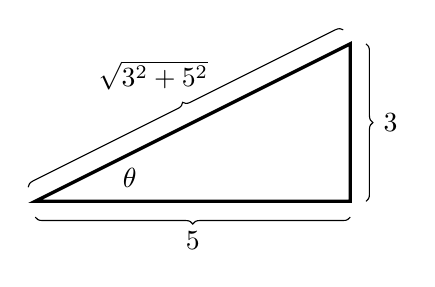
\begin{tikzpicture}
        \coordinate (C) at (0,2);
        \coordinate (D) at (4,2);
        \coordinate (E) at (4,4);
        \tkzMarkRightAngle(C,D,E)
        \tkzMarkAngle(D,C,E)
        \draw[decoration={brace,mirror,raise=.2cm},decorate,thin] (0,2)--(4,2);
        \draw[decoration={brace,mirror,raise=.2cm},decorate,thin] (4,2)--(4,4);
        \draw[decoration={brace,raise=.2cm},decorate,thin] (0,2)--(4,4);
        \draw[very thick] (D)--(E)--(C)--cycle;
        \node at (2,2-.5) {$5$};
        \node[anchor=west] at (4+.3,3) {$3$};
        \node at (2-.5,3+.6) {$\sqrt{3^2+5^2}$};
        \node at (1.2,2.3) {$\theta$};
      \end{tikzpicture}
    \end{image}
    From this triangle and our work above, we see that
    \[
    \sin(\theta) = \answer[given]{3/\sqrt{3^2+5^2}}.
    \]
  \end{explanation}
\end{example}



We'll also use the Pythagorean Theorem to help us simplify abstract
expressions into ones we can compute with ease.

\begin{example}
  Simplify
  \[
  \tan(\arccos(x))
  \]
  \begin{explanation}
    Start by saying
    \[
    \theta = \arccos(x)
    \]
    This means $\tan(\arccos(x)) = \tan(\theta)$. Apply cosine to both
    sides of the equation above,
    \begin{align*}
      \cos(\theta) &= \cos(\arccos(x))\\
      \cos(\theta) &= \answer[given]{x}.
    \end{align*}
    Now we will use the Pythagorean Theorem to deduce
    $\tan(\theta)$. If $\cos(\theta)=x$, the triangle in question must
    be similar to this triangle:
    \begin{image}[2in]
      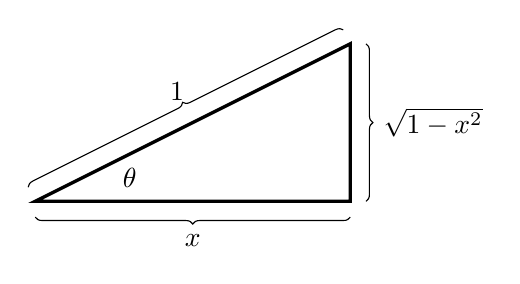
\begin{tikzpicture}
        \coordinate (C) at (0,2);
        \coordinate (D) at (4,2);
        \coordinate (E) at (4,4);
        \tkzMarkRightAngle(C,D,E)
        \tkzMarkAngle(D,C,E)
        \draw[decoration={brace,mirror,raise=.2cm},decorate,thin] (0,2)--(4,2);
        \draw[decoration={brace,mirror,raise=.2cm},decorate,thin] (4,2)--(4,4);
        \draw[decoration={brace,raise=.2cm},decorate,thin] (0,2)--(4,4);
        \draw[very thick] (D)--(E)--(C)--cycle;
        \node at (2,2-.5) {$x$};
        \node[anchor=west] at (4+.3,3) {$\sqrt{1-x^2}$};
        \node at (2-.2,3+.4) {$1$};
        \node at (1.2,2.3) {$\theta$};
      \end{tikzpicture}
    \end{image}
    From this triangle and our work above, we see that
    \[
    \tan(\arccos(x)) = \tan(\theta) = \answer[given]{\frac{\sqrt{1-x^2}}{x}}.
    \]
  \end{explanation}
\end{example}


\end{document}
